\section{Methods} \label{s:N_II:methods}

% Introduce the new pipeline 
% In the previous network chapters the graphs were generated using an adapted version of the PGCNA as it was for an initial exploration of the network approach to stratify a disease. 
The previous chapter represented an exploration and testing of the integrative network approach to stratify the MIBC and the implementation used a modified version of PGCNA package to build the networks. However, PGCNA was created with the goal to integrate multiple gene expression datasets at the network construction stage which is different from this project's goals. The main drawback of using PGCNA is that it was built to support Leiden as a community detection and the code structure was inflexible for enabling data integration. For this reason, a new package was developed in this PhD called \textit{iNet} with the following requirements: 

% Goals of the pipeline
\begin{itemize}
    \item Modular - easy to change and adapt the different stages of the network pipeline. This  is essential for data integration and future work
    \item Multiple community detection - apart from Leiden and SBM, it should be easy to adapt for future methods. This also includes the capability to specify the arguments for a community detection algorithm
    \item Weight modifiers - have the capability to easily add a new function to modify the weights
    \item Other correlation matrices - allow to easily change the correlation metric from which the co-expressed network is built
    \item Selective edge pruning - to easily change the genes that are prioritise in selective edge pruning 
    \item Readability - easy to understand and use by another Python programmer
\end{itemize}

Apart from following the Object Oriented Programming (OOP), splitting the process into different stages helped meeting the implementation requirements. Without delving into the code is split into following stages:
\begin{enumerate}
    \item Filter the data - keep the specified number of the genes with the highest median, median ratio
    \item Build the correlation matrix
    \item Apply the weight modifiers
    \item Edge pruning
    \item Apply community detection algorithm
    \item Save the output which are then analysed in separate Jupyter Notebooks
\end{enumerate}

% Highlight some of the changes
Compared to the previous network pipeline, the correlation matrix can be also be built from other correlation metrics such as the partial-correlation. The weight modifier function is easy to change and supports the sigmoid function to reward the mutated genes. The edge pruning uses the information from an input file of the genes that are allowed multiple edges. There is more freedom to change the community detection and configure them, apart from the \acrfull{sbm} support, the Leiden algorithm can be applied with Constant Pots Model as modularity maximisation function\footnote{Const Pots Model or CPM is an alternative cost function}.

% How was tested
The new package was tested by comparing the outputs generated with \textit{iNet} against those from the modified PGCNA pipeline. This was possible despite implementation differences as the two pipelines followed the same principles, where a correlation matrices is used to build the graph. This means, that both the correlation matrices and the generated networks could be used to test the implementation.

\subsection*{Reward modifier - sigmoid} \label{s:N_II:reward}

In previous chapter two different edges weight modifiers were introduced with the goal to integrate the mutation count at the weight level; see \cref{fig:N_I:modifiers}. It was observed that both had an effect on the network metrics but with little impact on the MIBC stratification. One possible explanation for this is that the modifiers had a steep increase/decrease over the weights with no intermediate effect to the weights. This means that only a few genes and their connections were affected.

The reward function is preferred over the penalised modifier as it did not contain isolated nodes. The initial version of the reward modifier is described by \cref{eq:n_II:norm3_func}, where w is the $log_2$ transformed of the mutation burden shifted by 1 (to avoid undefined values at 0 see \cref{eq:n_II:w} \footnote{\Cref{eq:n_II:w,eq:n_II:norm3_func} are the same equations as the ones from \cref{s:N_I:weight_modifiers} and were presented here again to improve the reading experience.}. $x$ represents the mutation burden taken from the TCGA dataset.  The behaviour of the function is shown by the red line in \cref{fig:N_II:modifiers_comp} which has an arc-like behaviour, where most of the mutated genes increase the weights value up to $50\%$ (value of $1.5$). The figure also shows that genes with high mutation burden do not have a proportional impact on the weight modifier.

\begin{equation} \label{eq:n_II:w}
    w(x) = \log_2(x+1)
\end{equation}

\begin{equation} \label{eq:n_II:norm3_func}
\text{f}(w) = \frac{\max(w) + w}{\max(w)}
\end{equation}

To accommodate the limitation of the previous function, a new reward function is introduced in this chapter as seen in \cref{eq:sig_func} which is modelled after the logistic function (with the sigmoid function being a special case of this). In this new reward function, $x$ represents the input variable, and $x_0$ shifts the function along the x-axis. The mutation counts are scaled to the range $[-12, 12]$, with $x_0 = -8$, and the constant $+1$ in \cref{eq:sig_func} keeps the values in the range $[1, 2]$. The parameters were determined empirically to ensure that the function meets the desired shape of a gradual increase.

\begin{equation} \label{eq:sig_func}
\text{f}(x) =  \frac{1}{1 + e^{-(x - x_0)}} + 1, \text{ where } x_0=-8
\end{equation}

The behaviour of the logistic reward function is represented by the green line in \cref{fig:N_II:modifiers_comp}. From the figure it can be noticed the gradual increase of the weight modifier with the mutational burden. Highly mutated genes sch as \textit{FGFR3, KMT2C, PIK3CA} have a much higher impact on the weights compared to the previous weight function. It worth noting that a 50\% increase of the weight value happens at a point of $\sim30$ mutation burden equating to $\sim7\%$ of the cohort mutated there are 112 genes mutated

Later in the chapter, \cref{s:N_II:reward_comp}, there is a direct comparison of the network metrics across both tumour and non-tumour of the two modifier functions.

\begin{figure}[H]    
    \centering
    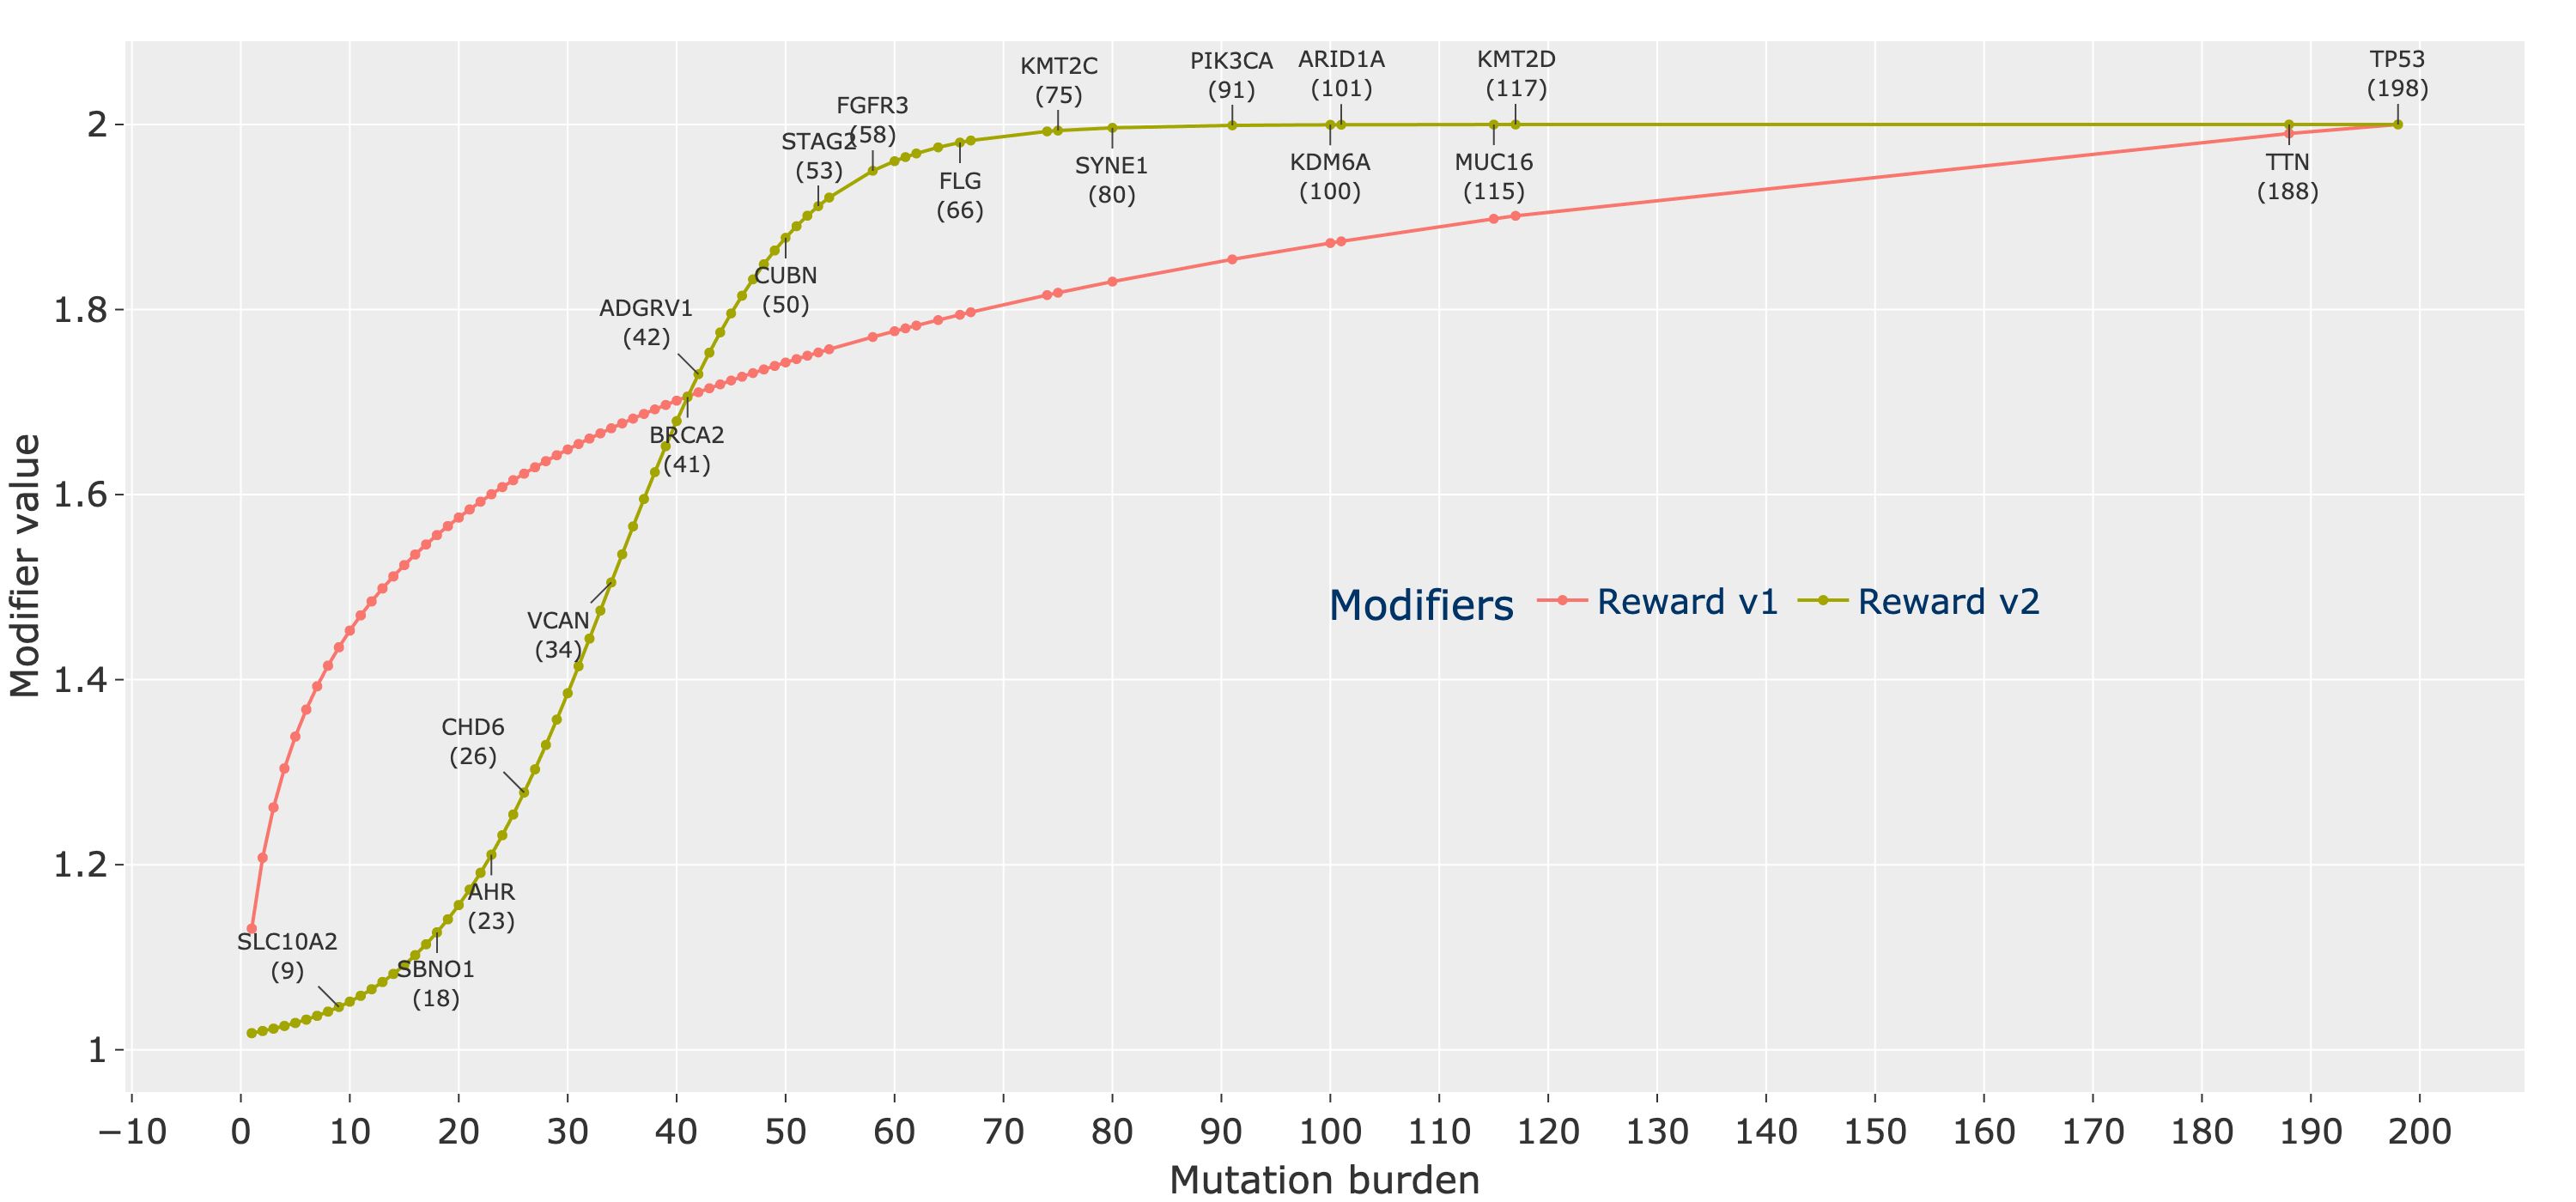
\includegraphics[width=1.0\textwidth,height=1.0\textheight,keepaspectratio]{Sections/Network_II/validation/reward_modifiers.png}
    \caption{The two reward modifiers explored in this project: Reward v1 (red) and Reward v2 (sigmoid). Both are shown over the mutation burden from TCGA. The points correspond to both of the plots but only shown on the Reward 2 line to avoid clutter. A value on the Y-axis of $1.2$ will mean that the weight is increased by $20\%$ where of $2$ will result in doubling it as it is the case for the highly mutated \textit{TP53} or \textit{TTN}. }
    \label{fig:N_II:modifiers_comp}
\end{figure}


% iMev
\subsection*{iMev - integrative MEV} \label{s:N_II:iMEV}

Module Evaluation Value or MEV was introduced in the PGCNA work from \citet{Care2019-ij} and covered in \cref{s:N_I:mev}. The role of the score is to bridge the gap between the gene to tumour representation by showing how much a sample is enriched by the (selected) gene expression from a community. This is done by summing up the z-scores of the $log_2$ gene expression in the community. Importantly, the gene expression  for the z-score has to always be from the dataset that is stratified which usually is the MIBC cohort from TCGA. This means that when the non-tumour dataset was used to generated the network, in \cref{s:N_II}, the gene expression of the non-tumour samples were not considered to inform the tumour subtyping. This can be accommodated by adapting the z-score.

\begin{equation} \label{eq:N_II:z_score}
z = \frac{x_{tum} - \mu_{tum}}{\sigma_{tum}}
\end{equation}

To calculate the z-score for the tumour dataset the equation in \cref{eq:N_II:z_score} is used, where $x_{tum}$ is the observed expression in a tumour sample, $\mu_{tum}$ and $\sigma_{tum}$ are the mean and standard expression across tumours. In the context of this project, the z-score measures how far the expression of a gene in a sample is from the mean expression across the tumours. Positive values denoting that the sample expression is higher than the mean while negative values indicating that is lower.


\begin{equation} \label{eq:N_II:i_z_score}
z = \frac{x_{tum} - \mu_{non\_tum}}{\sigma_{non\_tum}}
\end{equation}

The integrate the two gene expression datasets, the MEV score is changed to consider the expression trend in the non-tumour dataset but to use the sample observation from the tumour dataset; described by \cref{eq:N_II:i_z_score}. The change occurs at the mean and standard deviation which are now computed for the non-tumour samples or the dataset that it is used to generate the network; the observed samples, $x_{tum}$ remains unchanged. The modification of the z-score brings the distribution characteristics of the non-tumour dataset (or the data used to create the network) into the equation of computing the MEV. In other words, the equation \cref{eq:N_II:i_z_score} is computing how far is the gene expression in a tumour tumour sample with respect to the mean and standard deviation of the non-tumour.



